\documentclass[titlepage]{ltjsbook}
\usepackage[
  paperheight=232truemm, paperwidth=182truemm,
  top=20truemm, bottom=15truemm, inner=15truemm, outer=15truemm
  ]{geometry}

%\documentclass[tombow, paper={182truemm, 232truemm}, titlepage]{ltjsbook}
\usepackage{amsmath}
\usepackage{amsfonts}
\usepackage{amssymb}
\usepackage{mathtools}
\usepackage{mathrsfs}

\usepackage{textgreek}
\usepackage[luatex]{graphicx} 
%\usepackage[draft]{graphicx} % 画像が枠だけになる.
\usepackage{sidecap}
\usepackage[svgnames]{xcolor}
\usepackage{sty/julia-syntax-highlighting} % 
\usepackage{sty/indexing} % 

\usepackage[export]{sty/adjustbox} % added

\usepackage{fancyhdr}
\pagestyle{fancy}
\fancyfoot{}
\fancyhead[RO, LE]{\thepage}
\fancyhead[LO]{\nouppercase{\leftmark}}
\fancyhead[RE]{\nouppercase{\rightmark}}

%\renewcommand{\chaptermark}[1]{\markboth{#1}{} }
\renewcommand{\chaptermark}[1]{\markboth{第\ \thechapter\ 章. ~#1}{}}
% \renewcommand{\chaptermark}[1]{\markboth{\MakeUppercase{第\chaptername \thechapter 章.\ #1}}{}}
% \renewcommand{\headrulewidth}{0pt}
\usepackage{tcolorbox}
\usepackage{hyperref}
\usepackage{comment}

% https://ja.overleaf.com/learn/latex/Bibliography_management_with_bibtex
\usepackage[
    backend=biber,
    bibencoding=utf8,
    style=authoryear-comp, 
    url=false,
    isbn=true,
    doi=true,
    natbib=true, 
    alldates=year,
    maxcitenames=2,
    uniquelist=false, 
    sorting=ynt,
    sortcites=true,
    giveninits=true,
    terseinits=false,
    refsegment=chapter
]{biblatex}

\addbibresource{../references/07_bayesian-brain.bib}

\DeclareNameAlias{author}{last-first}
\AtEveryBibitem{\clearlist{language}}
\renewbibmacro{in:}{}

\newcommand{\jl}{\lstinline[language=julia]}

\title{\Huge \textbf{Juliaで作って学ぶ計算論的神経科学}}
\author{\huge 山本 拓都}
\date{\huge \today} 

\begin{document}
%\maketitle
\setcounter{tocdepth}{2}
\tableofcontents
\clearpage
\chapter{生成モデルとベイズ脳仮説}
%\section{推論的知覚と生成モデル}
%\subsection{逆問題と推論的知覚}
これまでの章では,知覚 (perception) のモデル,すなわち外界からの入力に対して,どのようにして神経回路網が意味のある出力を生成するのか,という問題を主に扱ってきた.ここで改めて知覚の基本的な定義を確認しておこう.知覚とは,外界からの刺激を感覚受容器によって受容し,それに意味を与える過程である.この「刺激に意味を与える」という個所を,より体系的に理解するために,「順問題」と「逆問題」という概念を導入しよう.

一般に,ある原因から結果を予測する問題は順問題 (forward problem) と呼ばれる.逆に,観測された結果からその原因を推定する問題は逆問題 (inverse problem) と呼ばれる.視覚を例にとって,順問題と逆問題について考えてみよう.たとえば,三次元の物体が光を反射し,それが二次元の網膜上にどのような像を結ぶか,という問いは順問題に分類される.これに対して,網膜上に投影された二次元像から,元の物体の三次元的な構造や大きさ,位置などを推定する課題が逆問題である\footnote{他にも逆問題は数多く存在する.逆問題は様々な分野に現れるが,ここでは医学や神経科学に関連した例として,外部から脳の構造や機能を推定する問題を取り上げる.たとえば,医用画像解析では,コンピュータ断層撮影 (computed tomography; CT) ,磁気共鳴画像法 (magnetic resonance imaging; MRI) ,陽電子放射断層撮影 (positron emission tomography; PET) などにおいて,観測データから画像を再構成する必要がある.この再構成処理には,CTやPETでは逆ラドン変換,MRIでは逆フーリエ変換が用いられる.また,神経活動を非侵襲的に計測する手法として,脳波 (electroencephalography; EEG) や脳磁図 (magnetoencephalography; MEG) がある.これらにおける電流源推定 (source localization) も典型的な逆問題である.EEGやMEGにおける順問題は,脳内の神経電流源の位置・方向・強度から,頭皮上の電極 (EEG) や磁場センサ (MEG) によって観測される電位や磁場分布を予測することである.一方,逆問題は,実際に観測された電位や磁場データから,神経電流源の空間的位置と活動を推定することである.この逆問題は不良設定 (ill-posed) であるため,安定的に解くには,MRIから得られた頭部の構造データに基づいて構築された順モデル (forward model) が必要となる.}.光学の分野では,それぞれの問題は順光学 (forward optics) ,逆光学 (inverse optics) と呼ばれている.逆問題は多くの場合,不良設定問題 (ill-posed problem) となる.すなわち,解が存在しない,解が一意に定まらない,あるいはわずかな誤差に対して解が大きく変化するといった性質をもつ\footnote{これに対して,良設定問題 (well-posed problem) とは,解が存在し,一意であり,かつ入力の変動に対して連続的に変化する (安定性をもつ) ような問題を指す.良設定問題では,入力データに小さなノイズや誤差が含まれていても,求められる解は大きく変わることなく,安定に計算することができる.}.例えば,先ほどの例であれば同じ2次元像を示す3次元物体は複数 (あるいは無数に) 存在する.そのため,逆問題を解くには,事前知識や仮定 (制約条件,正則化) の導入などが必要となる.

こうした逆問題を踏まえ,知覚とは単なる入力情報の受動的な処理ではなく,感覚入力という結果から外界に存在する潜在的な原因を推定する逆推論 (abductive reasoning) の過程とみなす考えがある \citep{helmholtz1867, mumford1992computational, kawato1993forward, friston2003learning}\footnote{Helmholtz は,知覚を単なる感覚の受容ではなく,感覚入力に意味を与え,対象として構成する過程であると捉えた.この過程には,観念の連合 (\textit{Vorstellungsverbindungen}) が関与している.観念の連合とは,過去の経験によって形成された (必ずしも言語化を伴わない) 観念や知識が,現在の感覚入力と結び付けられる過程を指す.通常,推論とは意識的に行われるものと考えられているが,Helmholtz はこのような観念の連合を,意識されることなく行われる推論として捉え,無意識的推論 (\textit{unbewusster Schluss}, unconscious inference)  と表現した.なお,この脚注ではドイツ語を斜体で表記した.}.この枠組みを推論的知覚 (perception as inference) と呼ぶ.推論的知覚は, 外界の潜在的な原因から感覚入力が生成される過程を記述する確率的生成モデル (probabilistic generative model) に基づいて説明される. 確率的生成モデルについて説明する前に,前提となるベイズ推論について次節で説明する.
%本章で触れる内容についてまとめ直す.

\begin{tcolorbox}
本章で触れる内容についてまとめ直す.
\end{tcolorbox}

\section{確率的生成モデル}
\subsection{確率的生成モデルとベイズ推論}
外界から感覚入力などを通じて観測データ $x$ を得る状況を考えよう\footnote{厳密には,確率変数は大文字 $X$,その実現値は小文字 $x$ で表記して区別するのが原則である. しかし,応用的な文脈では両者を混同しても支障をきたすことは少ないため,本書では明確に区別しない方針をとる. 特に,確率変数がスカラーの場合には大文字・小文字で容易に区別できるが,ベクトルや行列を扱う際には表記が煩雑となり,可読性を損ねる恐れがある. このため,本書では,確率変数とその実現値の区別が必要となる場合にはその旨を明示し,それ以外では変数の次元に基づく記号表記を基本とする. } . 観測データが存在するということは, それを生成する確率分布\footnote{本書では確率分布を確率密度関数の意味で用いる.} $p_{\mathrm{data}}(x)$ が存在する (すなわち $x \sim p_{\mathrm{data}}(x)$ である) と仮定できる. この $p_{\mathrm{data}}(\cdot)$ はしばしば真の確率分布と呼ばれるが, 実際にそのような分布が存在する保証はなく, 多くの場合は未知である. もし $p_{\mathrm{data}}(\cdot)$ が既知であれば, 任意のサンプル $x$ をそこから直接生成 (サンプリング) できるが, 現実にはこれを直接知ることはできない. 

このため, 観測データがある確率的な生成過程に従って生じたと仮定し, その過程を記述する生成モデルを構築する. 生成モデルは分布を明示的に表現するため, 新たなデータの生成や欠損値の補完, 潜在構造の抽出, 外界の状態推定など, 多様な推論を可能にする. ここではパラメータ $\theta$ をもつ条件付き確率密度関数 $p(x \mid \theta)$ を導入し, 観測の背後にある生成過程を近似的に表す. このような確率分布 $p(x \mid \theta)$ を定めるモデルを確率的生成モデル (probabilistic generative model) と呼ぶ. また, このように有限個のパラメータ $\theta$ で分布形状を規定するモデルをパラメトリックモデル (parametric model) と呼ぶ\footnote{有限個のパラメータで分布形状をあらかじめ規定せず, データ量に応じて表現可能な複雑さが変化するものをノンパラメトリックモデル (non-parametric model) と呼ぶ. 代表例にはヒストグラムやカーネル法による密度推定, ガウス過程, 分位点回帰などがある. 特に分位点回帰は分布型強化学習への応用を通じて神経科学とも関連し, その詳細は第9章で述べる. }. 

例えば, 正規分布 $p(x \mid \theta) = \mathcal{N}(x \mid \mu, \sigma^2)\quad \left(\theta = \{\mu, \sigma\}\right)$はパラメトリックな確率的生成モデルの一例である. この場合, 分布の形状 (正規分布) はあらかじめ固定され, 未知なのはパラメータ $\theta$ である. ここで改めて強調しておくと, 目標は真の分布 $p_{\mathrm{data}}(\cdot)$ を近似できる生成モデルを構築することである. パラメトリックモデルの場合, この目標はモデルのパラメータを適切に推定することによって達成される. 

パラメータ推定には, 大きく分けて二つの方法がある. 一つは, パラメータの最適な一点の値を求める点推定であり, もう一つはパラメータを確率変数として扱い, その不確実性を含めて推定する分布推定である. 
パラメータ推定には大きく二つの方法がある. 一つは, パラメータの最適な一点の値を求める点推定であり, もう一つはパラメータを確率変数として扱い, その不確実性を含めて推定する分布推定である. 分布推定には様々な方法があるが, ここではその代表例としてベイズ推論 (Bayesian inference) を取り上げる. ベイズ推論では, 観測前のパラメータ分布を事前分布 (prior) $p(\theta)$, 観測後の分布を事後分布 (posterior) $p(\theta \mid x)$ と呼び, 事前分布を事後分布へと更新する. この更新は, 尤度 (likelihood) とベイズの定理 (Bayes’ theorem) に基づいて行われる. 

\subsubsection{尤度}
先ほど導入した $p(x \mid \theta)$ は,観測データ $x$ とパラメータ $\theta$ のどちらを変数とみなすかによって確率モデルと尤度という2通りの解釈がある.

確率モデルとして解釈する場合,$\theta$ を固定し, $x$ を確率変数として扱う.このとき,$p(x \mid \theta)$ は「$\theta$ が与えられたときに, どのようなデータ $x$ がどの確率で得られるか」を表す. 

一方で,尤度として解釈する場合は,観測データを固定して, $\theta$ を変数として扱う.このとき,
\begin{equation}
L(\theta; x) \coloneq p(x \mid \theta)
\end{equation}
を尤度関数 (likelihood function) と呼ぶ. 尤度は, 仮定した $\theta$ の下でデータが得られる「尤もらしさ」を定量化する指標であり, 値が大きいほどデータをよく説明すると解釈できる. なお, 尤度関数は $\theta$ に関する確率分布ではないため, $\theta$ について積分しても必ずしも1にはならない. 

\subsubsection{ベイズの定理}
事前分布と尤度が設定されれば,事後分布を次式で表されるベイズの定理によって求めることができる: 
\begin{equation}
\underbrace{p(\theta \mid x)}_{\text{事後分布}} = \frac{\overbrace{p(x \mid \theta)}^{\text{尤度}}\, \overbrace{p(\theta)}^{\text{事前分布}}}{\underbrace{p(x)}_{\text{周辺尤度}}}
\end{equation}
ここで
\begin{equation}
p(x) = \int p(x \mid \theta)\, p(\theta)\, \mathrm{d}\theta
\end{equation}
は周辺尤度 (marginal likelihood) あるいは 証拠 (evidence) ,正規化定数 (normalization constant) と呼ばれる. このベイズの定理は
\begin{equation}
p(\theta, x) = p(x \mid \theta)\, p(\theta) = p(\theta \mid x)\, p(x)
\end{equation}
が成り立つことから導かれる.ここで $p(\theta, x)$ は $\theta$ と $x$ の同時確率分布 (joint probability distribution) である.

\subsubsection{予測分布}
事後分布 $p(\theta \mid x)$ は, 観測データを得た後のパラメータ $\theta$ の確率分布であり, ベイズ推論はこの分布を更新する過程とみなせる. 十分に更新された事後分布が得られれば, 新たなデータの予測も可能となる. 予測においては事後分布全体を平均化した事後予測分布 (posterior predictive distribution) を用いる. 観測されたデータの実現値を $x$, 予測対象のデータを $\tilde{x}$ とすると, 
\begin{align}
p(\tilde{x} \mid x)
&= \int p(\tilde{x}, \theta \mid x) \, \mathrm{d}\theta\\
&= \int p(\tilde{x} \mid \theta, x) \, p(\theta \mid x) \, \mathrm{d}\theta \\
&= \int p(\tilde{x} \mid \theta) \, p(\theta \mid x) \, \mathrm{d}\theta
\quad (\because \tilde{x} \perp\!\!\!\perp x \mid \theta)
\end{align}
となる. ここで最後の式変形には, 「$\theta$ が与えられた条件下で $\tilde{x}$ と $x$ が独立」という条件付き独立性を用いた. ベイズ推論において, この事後予測分布 $p(\tilde{x} \mid x)$ が真の生成分布の推論結果となる. なお,データの観測をしていない場合の予測は周辺尤度と同様の形式
\begin{equation}
p(\tilde{x}) = \int p(\tilde{x} \mid \theta)\, p(\theta)\, \mathrm{d}\theta
\end{equation}
で与えられ,これを事前予測分布 (prior predictive distribution) と呼ぶ.

\subsection{ベイズ線形回帰}
ここでは線形回帰モデルをベイズ化した,すなわち予測の不確実性を表現できるようにしたベイズ線形回帰 (Bayesian linear regression) モデルを取り扱う.

\subsubsection{多変量正規分布}
まず,多変量正規分布 (ガウス分布) を導入する.1次元の場合,正規分布は次の確率密度関数で表される.
\begin{equation}
\mathcal{N}(x \mid \mu, \sigma^2) 
\coloneq \frac{1}{\sqrt{2\pi \sigma^2}} \exp\left( -\frac{(x-\mu)^2}{2\sigma^2} \right)
\end{equation}
ここで,$\mu \in \mathbb{R}$ は平均,$\sigma^2 > 0$ は分散を表し,$\sigma$ は標準偏差である.この式を $x \in \mathbb{R}$ から $d$ 次元のベクトル $\mathbf{x} \in \mathbb{R}^d$ に拡張すると,分布は多変量正規分布 (multivariate normal distribution) となる.
\begin{equation}
\mathcal{N}(\mathbf{x} \mid \boldsymbol{\mu}, \boldsymbol{\Sigma}) 
\coloneq \frac{1}{\sqrt{(2\pi)^d \, |\boldsymbol{\Sigma}|}}
\exp\left( -\frac{1}{2} (\mathbf{x} - \boldsymbol{\mu})^\top \boldsymbol{\Sigma}^{-1} (\mathbf{x} - \boldsymbol{\mu}) \right)
\end{equation}
ここで,$\boldsymbol{\mu} \in \mathbb{R}^d$ は各成分の平均を並べた平均ベクトル,$\boldsymbol{\Sigma} \in \mathbb{R}^{d \times d}$ は共分散行列 (covariance matrix) である.共分散行列の対角成分は各次元の分散を表し,非対角成分は共分散を表す.このため,共分散行列は分散共分散行列 (variance-covariance matrix) とも呼ばれる.多変量正規分布が定義可能であるためには,$\boldsymbol{\Sigma}$ が正定値行列 (positive definite matrix) であることが必要であり,これは任意の非ゼロベクトル $\mathbf{z} \in \mathbb{R}^d \setminus \{\mathbf{0}\}$ に対して\footnote{集合 $A, B$ があるとき,$A \setminus B$ は$A$ から$B$ を引いた差集合を意味する.}
\begin{equation}
\mathbf{z}^\top \boldsymbol{\Sigma} \, \mathbf{z} > 0
\end{equation}
が成り立つことを意味する.この条件を満たす場合,$\boldsymbol{\Sigma}^{-1}$ が存在してそれ自体も正定値となるため,特に $\mathbf{x} = \boldsymbol{\mu}$ の場合も含めて
\begin{equation}
(\mathbf{x} - \boldsymbol{\mu})^\top \boldsymbol{\Sigma}^{-1} (\mathbf{x} - \boldsymbol{\mu}) \geq 0
\end{equation}
が常に成立する.なお,共分散行列は $\boldsymbol{\Sigma} = \boldsymbol{\Sigma}^\top$ という対称性を持つが,これは非対角成分が共分散を表し,その定義から $\boldsymbol{\Sigma}_{ij} = \boldsymbol{\Sigma}_{ji}$ が必ず成り立つことによる.正定値行列という概念は,対称行列や,より一般にはエルミート行列に対して定義されるため,多変量正規分布においても,共分散行列はこのように対称性を持った上で正定値でなければならない.Julia言語において,行列が正定値行列か確認するには \jl{LinearAlgebra} ライブラリの \jl{isposdef} 関数を用いればよい.行列 \jl{A} が正定値ならば,\jl{isposdef(A)} は\jl{true} を返す.

また,後ほど使用するため多変量正規分布の確率密度関数の対数を取った形式を確認しておこう.$p(\mathbf{x})=\mathcal{N}(\mathbf{x} \mid \boldsymbol{\mu}, \boldsymbol{\Sigma}) $ とすると,
\begin{equation}
\ln p(\mathbf{x}) = -\frac{d}{2} \ln (2\pi) - \frac{1}{2} \ln \lvert\boldsymbol{\Sigma}\rvert - \frac{1}{2}(\mathbf{x} - \boldsymbol{\mu})^\top \boldsymbol{\Sigma}^{-1} (\mathbf{x} - \boldsymbol{\mu})
\end{equation}
となる.

\begin{tcolorbox}
多変量正規分布のコード
\end{tcolorbox}

\subsubsection{ベイズ線形回帰のモデル定義}
入力 $\mathbf{x} \in \mathbb{R}^d$ から実数値出力 $y \in \mathbb{R}$ を予測するモデルを考える. 基底関数 (basis function) $\phi:\mathbb{R}^d \to \mathbb{R}^{d'}$ を導入し,入力を $\phi(\mathbf{x}) \in \mathbb{R}^{d'}$ に写像する. バイアス項を含める場合には,基底関数の1つの成分を常に1を返す定数関数として組み込むことにする. 訓練データを $\mathcal{D}=\{(\mathbf{x}_i, y_i)\}_{i=1}^n$ とすると,計画行列は
\begin{equation}
\Phi = 
\begin{bmatrix}
\phi(\mathbf{x}_1)^\top \\
\vdots \\
\phi(\mathbf{x}_n)^\top
\end{bmatrix}
\in \mathbb{R}^{n\times d'}
\end{equation}
で表される. 重みパラメータ $\mathbf{w}\in\mathbb{R}^{d'}$ を導入すると,$\mathbf{y}=[y_1,\dots,y_n]^\top \in \mathbb{R}^n$ の生成過程は
\begin{equation}
p(\mathbf{y}\mid \mathbf{w},\mathbf{X})
=\mathcal{N}\,\left(\mathbf{y}\mid \Phi \mathbf{w},\,\beta^{-1}\mathbf{I}_n\right)
= \prod_{i=1}^n \mathcal{N}\,\left(y_i\mid \phi(\mathbf{x}_i)^\top\mathbf{w} , \beta^{-1}\right)
\end{equation}
で与えられる.ここで,$\beta\,(>0)$ は尤度の精度 (precision) であり,分散の逆数を意味する.さらに,重みパラメータに対して正規分布の事前分布
\begin{equation}
p(\mathbf{w})=\mathcal{N}\,\left(\mathbf{w}\mid \mathbf{0},\alpha^{-1} \mathbf{I}_{d'}\right)
\end{equation}
を仮定する. ここで,$\alpha\,(>0)$ はパラメータの事前分布の精度である.また,この事前分布は共役事前分布 (conjugate prior) となっている. 共役であるとは,事前分布と尤度の組み合わせにより得られる事後分布が,同じ分布族で表現できることを意味する. 

\subsubsection{事後分布}
次に,事後分布を導出する.ベイズの定理より
\begin{equation}
p(\mathbf{w}\mid \mathbf{y},\mathbf{X}) \propto p(\mathbf{y}\mid \mathbf{w},\mathbf{X})\,p(\mathbf{w})
\end{equation}
が成り立つ\footnote{ここで,ベイズの定理における分母の周辺尤度 $p(\mathbf{y}\mid\mathbf{X})$ は事後分布 ($\mathbf{w}$の関数) の形状に影響しないため,無視した.また,$\mathbf{X}$ は常に実現値で与えられるので,$p(\mathbf{X})$ を考える必要はない.}.次に,事後分布を解析的に計算し,多変量正規分布の係数を無視した形状に式をまとめなおす.両辺の対数を取り,$\mathbf{w}$ に関する二次形式をまとめると次のようになる:
\begin{align}
\ln p(\mathbf{w}\mid \mathbf{y},\mathbf{X})
&\propto \ln p(\mathbf{y}\mid \mathbf{w},\mathbf{X}) + \ln p(\mathbf{w}) \\
&= -\frac{\beta}{2}\lVert \mathbf{y}-\Phi\mathbf{w}\rVert^2 -\frac{\alpha}{2}\lVert \mathbf{w}\rVert^2 + \text{const.}\\
&=-\frac{1}{2}\left[\mathbf{w}^\top\left(\beta\Phi^\top\Phi+\alpha\mathbf{I}_{d'}\right)\mathbf{w}-2\beta\mathbf{y}^\top\Phi\mathbf{w}\right]+ \text{const.}
\end{align}
が成り立つ ($\mathbf{w}$ を含まない項は $\mathrm{const.}$ に吸収した).ここで,事後分布を $\mathbf{w}$ についての多変量正規分布として
\begin{equation}
p(\mathbf{w} \mid \mathbf{y}, \mathbf{X}) \coloneq \mathcal{N}(\mathbf{w}\mid \hat{\boldsymbol{\mu}}, \hat{\boldsymbol{\Sigma}})
\end{equation}
とおく.この確率密度関数の指数部 ($\exp(\cdot)$ の中身) は
\begin{equation}
-\frac{1}{2}(\mathbf{w}-\hat{\boldsymbol{\mu}})^\top \hat{\boldsymbol{\Sigma}}^{-1} (\mathbf{w}-\hat{\boldsymbol{\mu}})
= -\frac{1}{2}\left[\mathbf{w}^\top \hat{\boldsymbol{\Sigma}}^{-1} \mathbf{w}
- 2 \hat{\boldsymbol{\mu}}^\top \hat{\boldsymbol{\Sigma}}^{-1} \mathbf{w}
+ \hat{\boldsymbol{\mu}}^\top \hat{\boldsymbol{\Sigma}}^{-1} \hat{\boldsymbol{\mu}}\right]
\end{equation}
であるため,$\mathbf{w}$ を含む項のみに関して両者を比べると,
\begin{equation}
\hat{\boldsymbol{\Sigma}}^{-1}=\beta\Phi^\top\Phi+\alpha\mathbf{I}_{d'},\quad \hat{\boldsymbol{\mu}}=\hat{\boldsymbol{\Sigma}}\beta\mathbf{y}^\top\Phi
\end{equation}
とすれば良いことが分かる.

\subsubsection{事後予測分布}
最後に,事後予測分布の導出を行う.新しい入力を $\tilde{\mathbf{x}}$,対応する出力を $\tilde{y}$ で表す.事後予測分布は前節での導出に基づくと,
\begin{equation}
p(\tilde{y} \mid \tilde{\mathbf{x}},\mathbf{y},\mathbf{X})=\int p(\tilde{y}\mid \mathbf{w},\tilde{\mathbf{x}})\,p(\mathbf{w}\mid \mathbf{y},\mathbf{X})\,\mathrm{d}\mathbf{w}
\end{equation}
により計算することができる.ここで,生成過程の仮定より
\begin{equation}
p(\tilde{y}\mid \mathbf{w},\tilde{\mathbf{x}})=\mathcal{N}\left(\tilde{y}\mid  \phi(\tilde{\mathbf{x}})^\top\mathbf{w}, \beta^{-1}\right)
\end{equation}
である.積分を直接実行すると煩雑な計算を要するため, ここでは正規分布の閉じた性質を利用する. すなわち, 正規分布を正規分布で畳み込むと再び正規分布となる. このため, 事後予測分布は平均と分散を計算するだけで決定できる. 
\begin{align}
\mathrm{E}[\tilde{y}]&=\mathrm{E}_{\mathbf{w}} \left[\mathrm{E}[\tilde{y} \mid \mathbf{w}] \right]=\mathrm{E}_{\mathbf{w}} \left[\phi(\tilde{\mathbf{x}})^\top\mathbf{w} \right]=\phi(\tilde{\mathbf{x}})^\top\mathrm{E}[\mathbf{w}]=\phi(\tilde{\mathbf{x}})^\top\hat{\boldsymbol{\mu}}\\
\mathrm{Var}[\tilde{y}] &= \mathrm{E}_{\mathbf{w}}\left[ \mathrm{Var}[\tilde{y}\mid \mathbf{w}] \right] + \mathrm{Var}_{\mathbf{w}}\left[ \mathrm{E}[\tilde{y} \mid \mathbf{w}] \right]=\mathrm{E}_{\mathbf{w}}\left[\beta^{-1} \right] + \mathrm{Var}_{\mathbf{w}}\left[\phi(\tilde{\mathbf{x}})^\top\mathbf{w} \right]\\
&=\beta^{-1}+\phi(\tilde{\mathbf{x}})\,\mathrm{Var}[\mathbf{w}]\,\phi(\tilde{\mathbf{x}})^\top=\beta^{-1}+\phi(\tilde{\mathbf{x}})^\top\hat{\boldsymbol{\Sigma}} \phi(\tilde{\mathbf{x}})
\end{align}
ここで,期待値の計算では,期待値の線形性の法則を用いた.分散の計算では,全分散の法則 (law of total variance) および分散の線形変換の法則を用いた
\footnote{ここで用いた3つの法則を補足しておく.確率変数 $X, Y$ と行列 $\mathbf{A}$ に関して,以下の基本的な性質が成り立つ:
\begin{alignat*}{2}
&\textbf{(1) 期待値の線形性:} 
&&\quad \mathrm{E}[\mathbf{A}X] = \mathbf{A}\,\mathrm{E}[X] \\
&\textbf{(2) 全分散の法則 (分散分解の法則) :} 
&&\quad \mathrm{Var}[Y] = \mathrm{E}\!\left[\mathrm{Var}[Y\mid X]\right] 
   + \mathrm{Var}\!\left[\mathrm{E}[Y\mid X]\right] \\
&\textbf{(3) 分散の線形変換:} 
&&\quad \mathrm{Var}[\mathbf{A}X] = \mathbf{A}\,\mathrm{Var}[X]\,\mathbf{A}^\top
\end{alignat*}
}.
よって,事後予測分布は
\begin{equation}
p(\tilde{y} \mid \tilde{\mathbf{x}},\mathbf{y},\mathbf{X})\coloneq\mathcal{N}\left(\tilde{y}\;\middle\vert\; \phi(\tilde{\mathbf{x}})^\top\hat{\boldsymbol{\mu}},\,\beta^{-1}+\phi(\tilde{\mathbf{x}})^\top\hat{\boldsymbol{\Sigma}} \phi(\tilde{\mathbf{x}})\right)
\end{equation}
となる.

\begin{tcolorbox}
ベイズ線形回帰のコード
\end{tcolorbox}

\subsection{最尤推定とMAP推定}
ベイズ推論の枠組みから派生し,パラメータ $\theta$ の分布を推定するのではなく,その点推定値を与える手法について説明する.ここでは,パラメータの不確実性は扱わず,単一の推定値を得ること,すなわちパラメータの点推定について取り扱う.代表的な点推定の方法には,最尤推定 (maximum likelihood estimation; MLE) と 最大事後確率推定 (maximum a posteriori estimation; MAP推定) がある.

まず,一般的な生成モデルを考える.観測データを $\mathbf{x}$,未知パラメータを $\theta$,真のデータ分布を $p_{\mathrm{data}}(\mathbf{x})$,確率モデルあるいは尤度を $p(\mathbf{x}\mid \theta)$,事前分布を $p(\theta)$ とする.このとき,事後分布はベイズの定理により $p(\theta \mid \mathbf{x}) \propto p(\mathbf{x}\mid \theta)\,p(\theta)$ と表される.この設定の下で,各推定法におけるパラメータの推定値は次のように定式化できる:
\begin{alignat}{3}
\text{最尤推定:} &\quad \hat{\theta}_{\mathrm{ML}}\,&=\, \arg\max_{\theta} p(\mathbf{x} \mid \theta) &= \arg\max_{\theta}\, \ln p(\mathbf{x} \mid \theta)\\
\text{MAP推定:} &\quad \hat{\theta}_{\mathrm{MAP}}\,&=\, \arg\max_{\theta} p(\theta \mid \mathbf{x}) &= \arg\max_{\theta}\,\left[\ln p(\mathbf{x} \mid \theta) + \ln p(\theta)\right]
\end{alignat}
両者はよく似た形をしているが,最大化する対象 (目的関数) が異なる.最尤推定は尤度そのものを最大化するのに対し,MAP推定は事前分布を考慮した事後分布を最大化する.なお,最後の式変形では,$\theta$ に依存しない周辺尤度 $p(\mathbf{x})$ が最適化に影響しないことを利用している.

最尤推定に関しては,次のような最小化問題からの導出も可能である.生成モデルの学習における目的は,パラメータ $\theta$ を調整して,生成モデルが定める確率密度関数 $p(\mathbf{x} \mid \theta)$ を,学習データが従う真の分布 $p_{\mathrm{data}}(\mathbf{x})$ に近づけることである.この「近づける」という操作には,両分布間の差異を定量化する指標,すなわち確率分布間の距離 (あるいは不一致度) を定義する必要がある.ここではその尺度として,KLダイバージェンス (Kullback–Leibler divergence) を用いる:
\begin{equation}
D_{\mathrm{KL}}\left(p_{\mathrm{data}}(\mathbf{x}) \,\Vert\, p(\mathbf{x} \mid \theta)\right)
\coloneq \int p_{\mathrm{data}}(\mathbf{x}) \ln \frac{p_{\mathrm{data}}(\mathbf{x})}{p(\mathbf{x}\mid \theta)} \, d\mathbf{x}
\end{equation}
この量は,真の分布 $p_{\mathrm{data}}(\mathbf{x})$ を基準としたときに,モデル分布 $p(\mathbf{x}\mid \theta)$ がどれだけ情報的に乖離しているかを測る指標である.すなわち,モデルが生成する分布が,実際のデータ分布からどの程度逸脱しているかを定量化するものである.このKLダイバージェンスを展開すると,
\begin{align}
D_{\mathrm{KL}}\left(p_{\mathrm{data}}(\mathbf{x}) \,\Vert\, p(\mathbf{x}\mid \theta)\right)
&= \int p_{\mathrm{data}}(\mathbf{x}) \ln p_{\mathrm{data}}(\mathbf{x}) \, d\mathbf{x} 
\ - \int p_{\mathrm{data}}(\mathbf{x}) \ln p(\mathbf{x}\mid \theta) \, d\mathbf{x} \\
&= \text{const.} - \mathbb{E}_{\mathbf{x} \sim p_{\mathrm{data}}} \left[ \ln p(\mathbf{x}\mid \theta) \right]
\end{align}
となる.ここで第1項は $\theta$ に依存しない定数であるため,パラメータ $\theta$ を最適化する際には,第2項の期待値 (すなわち対数尤度の期待値) を最大化することに等しい.したがって,最適なパラメータ $\theta^*$ は,
\begin{equation}
\theta^* = \arg\min_\theta D_{\mathrm{KL}}\left(p_{\mathrm{data}}(\mathbf{x}) \,\Vert\, p(\mathbf{x}\mid \theta)\right)
= \arg\max_\theta \mathbb{E}_{\mathbf{x} \sim p_{\mathrm{data}}} \left[ \ln p(\mathbf{x}\mid \theta) \right]
\end{equation}
として求められる.しかし実際には,真の分布 $p_{\mathrm{data}}(\mathbf{x})$ の形は不明であり,観測されるのは有限個のデータ点 $\{\mathbf{x}_i\}_{i=1}^n$ のみである.そこで,真の分布の代替として,以下のような経験分布 (empirical distribution)  $\hat{p}_{\mathrm{data}}(\mathbf{x})$ を用いる:
\begin{equation}
\hat{p}_{\mathrm{data}}(\mathbf{x}) \coloneq \frac{1}{n} \sum_{i=1}^n \delta(\mathbf{x} - \mathbf{x}_i)
\end{equation}
ここで,$\delta(\cdot)$ は Dirac のデルタ関数であり,この経験分布 $\hat{p}_{\mathrm{data}}(\mathbf{x})$ は,観測された各データ点の位置にのみ確率を集中させるような離散的な点分布として解釈できる.すなわち, サンプル $\{\mathbf{x}_i\}_{i=1}^n$ 以外の点では確率密度がゼロであり, 各 $\mathbf{x}_i$ に等しい重み $1/n$ を割り当てているとみなせる.この近似を用いることで,最適化問題は次のように書き換えられる:
\begin{equation}
\theta^* \approx \arg\max_\theta \mathbb{E}_{\mathbf{x} \sim \hat{p}_{\mathrm{data}}} \left[ \ln p(\mathbf{x}\mid \theta) \right]
= \arg\max_\theta \sum_{i=1}^n \ln p(\mathbf{x}_i \mid \theta)
\end{equation}
この最適化は最尤推定と一致する. 

一方で,MAP推定はこの枠組みに事前分布に基づく項を加えたものであり,「正則化付き最尤推定」とみなすことができる. さらに後に述べるように,MAP推定は変分推論 (variational inference) の特殊な場合 (近似分布をデルタ分布に制限した場合) として位置づけることもできる. 本節では扱わず,変分推論の議論の後に改めて説明する. 

前項で説明したベイズ線形回帰モデルに対し,パラメータの最尤推定とMAP推定に基づいた推定を行ってみよう.それぞれの推定における最適化問題は,以下のように表すことができる.
\begin{align}
\hat{\mathbf{w}}_{\mathrm{ML}}\,&=\, \arg\max_{\mathbf{w}} p(\mathbf{y} \mid \mathbf{w}, \mathbf{X}) = \arg\max_{\mathbf{w}}\, \ln p(\mathbf{y} \mid \mathbf{w}, \mathbf{X})\\
\hat{\mathbf{w}}_{\mathrm{MAP}}\,&=\, \arg\max_{\mathbf{w}} p(\mathbf{w} \mid \mathbf{y}, \mathbf{X}) = \arg\max_{\mathbf{w}}\, \left[\ln p(\mathbf{y} \mid \mathbf{w}, \mathbf{X})+ \ln p(\mathbf{w})\right]
\end{align}
まず,最尤推定の場合,対数尤度は
\begin{equation}
\ln p(\mathbf{y} \mid \mathbf{w}, \mathbf{X})=-\frac{\beta}{2}\lVert \mathbf{y}-\Phi\mathbf{w}\rVert^2 + \text{const.}
\end{equation}
であったので,最適化問題は
\begin{equation}
\arg\max_{\mathbf{w}}\,\ln p(\mathbf{y} \mid \mathbf{w}, \mathbf{X})=\arg\min_{\mathbf{w}}\,\lVert \mathbf{y}-\Phi\mathbf{w}\rVert^2
\end{equation}
となる.これは最小二乗法に一致し,通常の(ベイズでない)線形回帰モデルと同じ解を与える.

次に,MAP推定の場合,対数尤度に関しては上と同様であるため,対数事前分布 $\ln p(\mathbf{w})$ のみを考える.前項では事前分布を正規分布 $p(\mathbf{w})=\mathcal{N}\,\left(\mathbf{w}\mid \mathbf{0},\alpha^{-1} \mathbf{I}_{d'}\right)$ と設定したため,
\begin{equation}
\ln p(\mathbf{w}) = -\frac{\alpha}{2}\lVert \mathbf{w}\rVert^2 + \text{const.}
\end{equation}
であった.このため,最適化問題は対数尤度と合わせて,
\begin{equation}
\arg\max_{\mathbf{w}} p(\mathbf{w} \mid \mathbf{y}, \mathbf{X}) =\arg\min_{\mathbf{w}}\, \left[\lVert \mathbf{y}-\Phi\mathbf{w}\rVert^2 + \lambda \lVert \mathbf{w}\rVert^2 \right]
\end{equation}
となる.ただし,$\lambda = \alpha / \beta\, (>0)$ とした.この $\lambda$ は正則化の強度を表すハイパーパラメータである.よって,この最適化問題は最小二乗法の目的関数に,パラメータの二乗和 ($L^2$ノルムの二乗) を正則化項(罰則項)として追加したものであり,これはRidge回帰と一致する.

ここで,事前分布をラプラス分布にする場合を考える.ラプラス分布の確率密度関数は $x\in \mathbb{R}$ について,
\begin{equation}
\textrm{Lap}(x\mid \mu, b):=\dfrac{1}{2b}\exp\left(-\dfrac{\lvert x-\mu\rvert}{b}\right)
\end{equation}
で与えられる.ここで,$p(w_i)=\textrm{Lap}(w_i \mid 0, 2\alpha^{-1})=\dfrac{\alpha}{4}\exp\left(-\dfrac{\alpha}{2} \lvert w_i\rvert \right)$ に設定した場合は
\begin{equation}
\ln p(\mathbf{w}) = -\frac{\alpha}{2} \sum_{i=1}^n \lvert w_i\rvert+ \text{const.}
\end{equation}
となる.$L^1$ ノルムを $\lVert \mathbf{w}\rVert _1 := \sum_{i=1}^n \lvert w_i\rvert$ とすると,最適化問題は
\begin{equation}
\arg\max_{\mathbf{w}} p(\mathbf{w} \mid \mathbf{y}, \mathbf{X}) =\arg\min_{\mathbf{w}}\, \left[\lVert \mathbf{y}-\Phi\mathbf{w}\rVert^2 + \lambda\lVert \mathbf{w}\rVert _1 \right]
\end{equation}
と書ける.この最適化問題は最小二乗法の目的関数に,パラメータの絶対値 ($L^1$ノルム) を正則化項として追加したものであり,これはLasso回帰と一致する.

以上より,最尤推定は最小二乗法に一致し,MAP推定では事前分布の選択に応じてRidge回帰やLasso回帰と対応づけられる。すなわち,正則化はパラメータに対する事前分布の設定として解釈できる。

\subsection{潜在変数モデル}
ここで,$p_\theta(\mathbf{x})$ は,観測変数 $\mathbf{x}$ に対する条件付き分布 $p(\mathbf{x} \mid \theta)$ の略記である.

確率的主成分分析
\subsubsection{エネルギーベースモデル}

\subsection{階層ベイズモデル}

\section{スパース符号化と予測符号化}

\subsection{スパース符号化}


\begin{tcolorbox}
スパース符号化のコード
\end{tcolorbox}

\subsection{予測符号化}
\begin{tcolorbox}
予測符号化のコード
\end{tcolorbox}

\section{近似ベイズ推論}


\begin{SCfigure}[1.5][htbp]
  \centering
  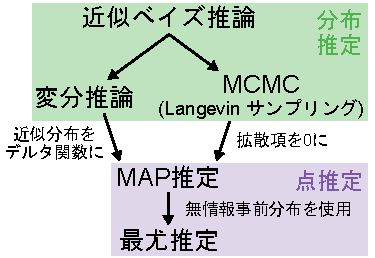
\includegraphics[width=0.4\textwidth]{./figures/approx_bayesian.pdf}
  \caption{分布推論から点推定への流れ}
  \label{fig:approx_bayesian}
\end{SCfigure}

\subsection{変分推論}
MAP推定は変分推論から導出できる.


\subsection{自由エネルギー原理}
FEP

Active inference
%A tutorial on the free-energy framework for modelling perception and learning
%What does the free energy principle tell us about the brain?

\subsection{マルコフ連鎖モンテカルロ法}
\subsubsection{ボルツマンマシン}

\section{神経回路による不確実性の表現}
\subsection{神経サンプリング}

\subsection{確率的集団符号化}

\printbibliography[segment=\therefsegment,heading=subbibliography,title={参考文献}]
\addcontentsline{toc}{section}{参考文献}
\end{document}